\documentclass[russian, 10pt]{beamer}

\usetheme{Madrid}
\usecolortheme{default}

\usepackage[utf8]{inputenc}
\usepackage[russian]{babel}
%\usepackage[T2A]{fontenc}

\usepackage{textcomp}
%\usepackage{a4wide}
\usepackage{bm}
\usepackage{caption}
\usepackage{subfig}
\usepackage{listings}
\usepackage{hyperref}
\usepackage{pgfplots}
\usepackage{tikz}
\usepackage{amsthm}
\usepackage{pgf,pgfarrows,pgfnodes}
\usepackage{amsmath}
\usepackage{amsfonts}
\usepackage{amssymb}
\usepackage{wrapfig}
\usepackage{indentfirst}
\usepackage{setspace}
\usepackage{graphicx}
\usepackage{textcomp}
\usepackage{array}

\usetikzlibrary{fit}
\usetikzlibrary{arrows.meta}
\usepackage{array, multirow}

\DeclareMathOperator{\E}{\mathbb{E}}
\DeclareMathOperator{\D}{\mathbb{D}}
\DeclareMathOperator{\R}{\mathbb{R}}


\usepackage{graphicx}
\usepackage[linesnumbered]{algorithm2e}

\title[Методы визуализации]
{
Задача Ticket ML Contest
}

\author[Бобров Евгений]{Бобров Евгений}
\institute[МГУ, ВМК]{
  {\scriptsize Московский государственный университет имени М.В. Ломоносова}\\
  {\scriptsize Факультет вычислительной математики и кибернетики}\\
  {\scriptsize Кафедра математических методов прогнозирования}\\
  
}


\date{15 ноября 2017}

\begin{document}

\begin{frame}
\maketitle
\end{frame}


\begin{frame}


\begin{figure}[htp]
\centering
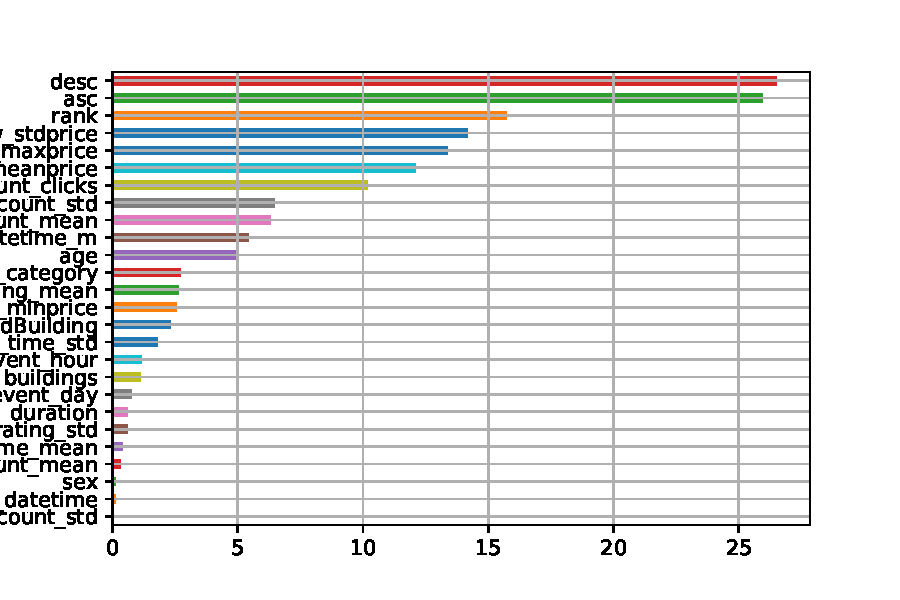
\includegraphics[scale=0.7]{auc.pdf}
\caption{Рассчёт важности признаков через roc-auc}
\end{figure}



\end{frame}

\begin{frame}

\begin{figure}[htp]
\centering
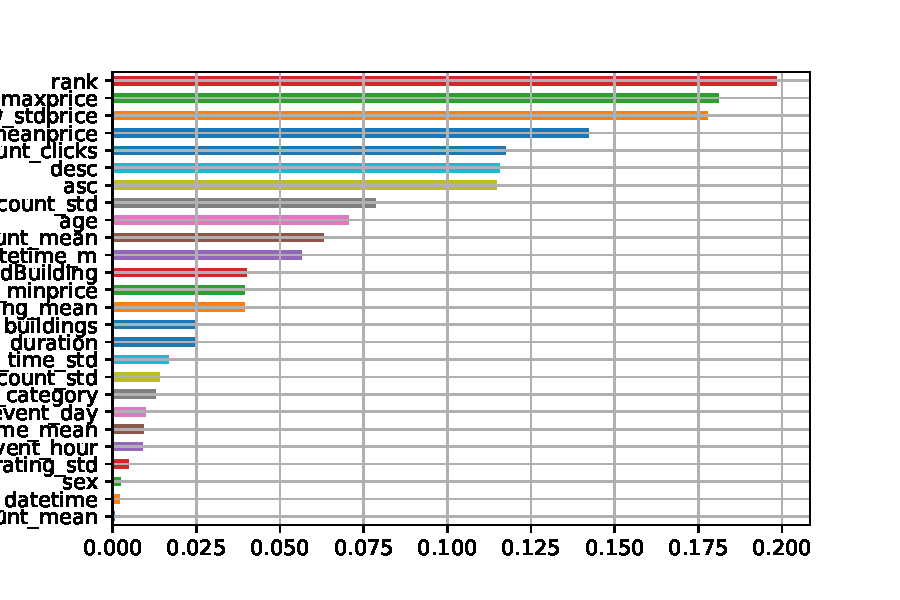
\includegraphics[scale=0.7]{cor.pdf}
\caption{Рассчёт важности признаков через корреляцию}
\label{}
\end{figure}




\end{frame}

\begin{frame}

\begin{figure}[htp]
\centering
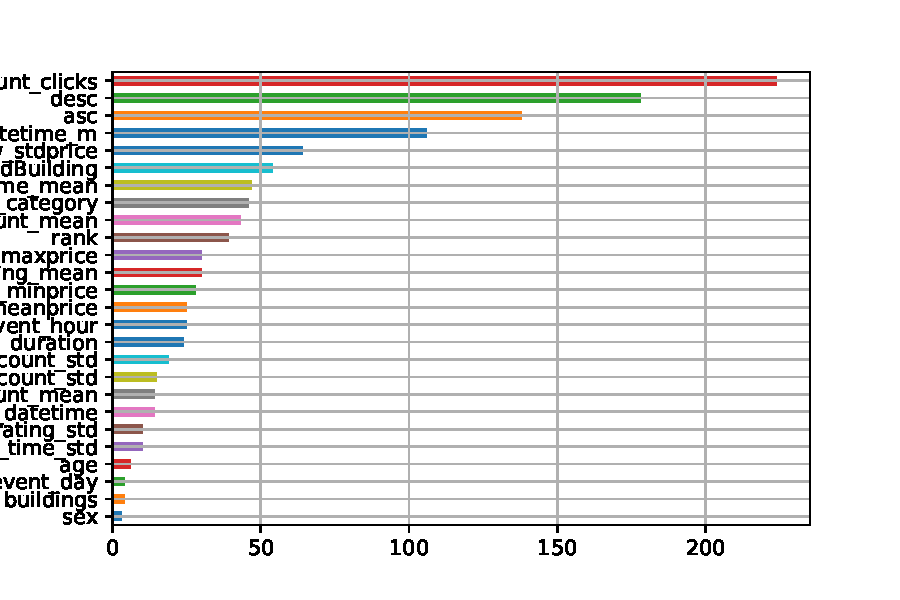
\includegraphics[scale=0.7]{splits.pdf}
\caption{Рассчёт важности признаков через число сплитов}
\end{figure}




\end{frame}




\end{document}